% Optimization Project: Biscuit Optimizer
% Roberto Basla
% Politecnico di Milano
% A.Y. 2021/2022

\section{Introduction}
This document reports the project developed for the Optimization course.

\subsection{The problem}
The problem consists in choosing how to place cookie cutters on some available dough in order to maximize the value assigned to each shape. Moreover, the most frequent shape must be selected no more than 3 times the most infrequent to avoid selecting too many biscuits of one type only.

This is a case of nesting problem, i.e. a two-dimensional cutting and packing problem involving irregular shapes; however, differently from classical formulations that define the elements to be placed as polygons, this project tackles the problem by considering images and binary masks over their pixels. The input data is preprocessed as follows.

\subsubsection{Available dough}
The available dough is represented by an image $P \in \mathbb{R}^{n \times m \times 3}$, where $n$ and $m$ are respectively the number of rows and columns, while $3$ refers to the color channels. The photo used for this project (\href{https://www.buttalapasta.it/ricette/ricetta-biscotti-al-latte/25247/}{source}) was cropped and subsampled (from the initial $n=180$, $m=192$ to $n=125$ and $m=134$) in order to simplify the problem. From this image, a binary mask encoding the usable area was manually drawn, thus obtaining the Dough bitmask $B \in \{0, 1\}^{n \times m}$ in Figure \ref{fig:input_dough}.

\begin{figure}[H]
	\centering	
	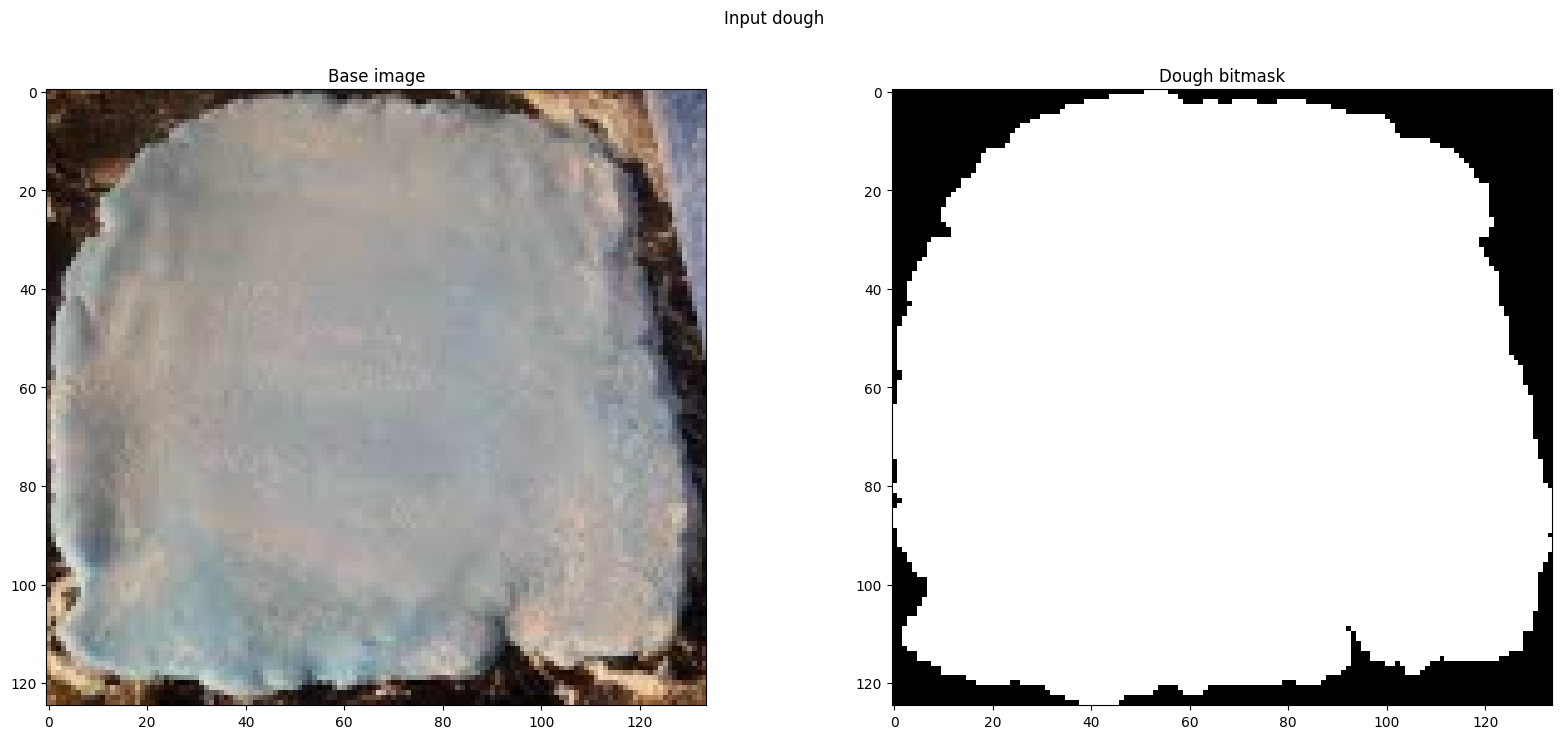
\includegraphics[width=\textwidth, keepaspectratio]{01-intro/subsampled_dough}
	\caption{Input dough and its binary mask (134×125 pixels)}
	\label{fig:input_dough}
\end{figure}

\subsubsection{Cookie cutters}
Cutter masks were hand drawn and assigned arbitrary values, as per Figure \ref{fig:cutters}; they will be the cookie cutters that need to be overlayed to the input image to "cut" it and obtain the final biscuits. These bitmasks will be referenced as $b_i$, while each pixel corresponds to $b_{i, h, k} \quad \forall h \in R_i, \forall k \in C_i$, where $R_i$ and $C_i$ represent respectively the set of rows and the set of columns of bitmask $i$.

\begin{figure}[H]
	\centering	
	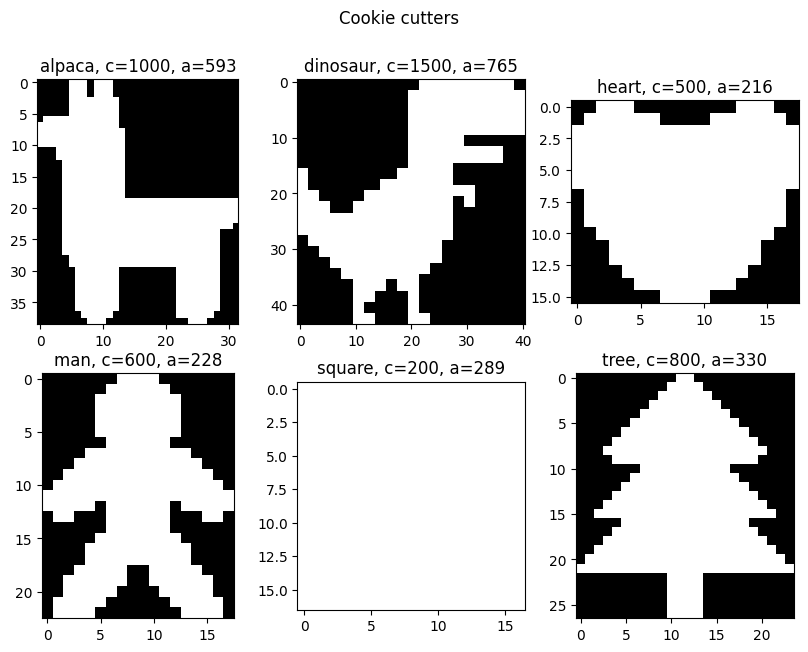
\includegraphics[width=.7\textwidth, keepaspectratio]{01-intro/cutters}
	\caption{Cutters' binary masks}
	\label{fig:cutters}
\end{figure}

\subsection{Technology}
This project was developed with both AMPL and Jupyter Notebooks using the following technologies:
\begin{itemize}[itemsep=-1mm, topsep=-1mm]
	\item AMPL with CPLEX solver
	\item Python with Google's OR-Tools optimization suite and CP-SAT solver
	\item Python with Gurobi's API and solver
	\item Pure Python for heuristics
\end{itemize}

All algorithms were run on a desktop setup with an Intel Core i7-6700 processor and 16GB DDR3 RAM; Python 3.9.12 was installed inside a Windows 10 Anaconda Environment.
